\documentclass{article}
\usepackage{graphicx}
\usepackage[margin=1in]{geometry}
\usepackage{indentfirst}

\begin{document}
\title{Project Testing and Delivery Document}
\author{Team D}
\date{\today}

\maketitle

\vspace*{3.5in}
\begin{table}[htbp]
\caption{Team}
\begin{center}
\begin{tabular}{|r | c|}
\hline
Name & ID Number \\
\hline\hline
Stefanie Lavoie & 1951750 \\
Pinsonn Laverdure & 9684352 \\
Ghislain Ledoux & 6376320 \\
Rigil Malubay & 6262732 \\
Philippe Milot & 9164111 \\
Christopher Mukherjee & 6291929 \\
\hline
\end{tabular}
\end{center}
\end{table}

\pagenumbering{gobble}% Remove page numbers (and reset to 1)
\clearpage

\begin{table}[htbp]
\caption{Revision History}
\begin{center}
\begin{tabular}{|c | c | c | c| }
\hline
Date & Version & Description & Author \\
\hline\hline
30/07/13 & 0.1 & Set up initial layout of deliverable & Philippe Milot \\
\hline
30/07/13 & 0.2 & Finished Section 2.2.1 & Philippe Milot \\
\hline
30/07/13 & 0.28 & Worked on Section 4 (almost complete) & Christopher Mukherjee \\
\hline
30/07/13 & 0.38 & Finished Section 1 & Christopher Mukherjee \\
\hline
04/08/13 & 0.39 & Started Section 3.2 & Stefanie Lavoie \\
\hline
06/08/13 & 0.41 & Finished Section 4 & Christopher Mukherjee \\
\hline
\end{tabular}
\end{center}
\end{table}

\clearpage

\tableofcontents
\clearpage

\pagenumbering{arabic}% Arabic page numbers (and reset to 1)

\section{Introduction} % COMPLETE

% [The introduction of the document provides an overview of the entire document, briefly introducing what are its goals, and what information is to be found in it.]

This document will describe in detail the testing process and final delivery for the Vessel Monitoring System which was developed in the context of the COMP354 course. This document includes a report on which items were tested and which were not, descriptions of the unit testing and requirements testing that was performed, a description of stress testing that could have been performed (but was \emph{NOT} performed), an installation manual and users manual, and a final cost estimation for the entire project.

\break

\section{Testing Report}

% [This section presents all the testing activities undertaken on the final product, as well as all the individual test cases used.]

\subsection{Test Coverage}

\subsubsection{Tested Items}

% [List all tested items, along with the test cases that were applied on this item. For each test item, explain why it was necessary to test it. For instance, all features listed as requirements for each build is a mandatory test item. In addition, identify at least five units (i.e. classes/methods) and explain why they require unit testing due to their importance in the implementation through their frequency of use and/or the severity of the impact of their misbehavior. You can categorize your tested items, e.g. “Requirements”, “Units”, etc.]

\subsubsection{Untested Items of Interest}

% [List all untested items that you find would necessitate testing. Explain how it could be tested, and why it would be important to test.]

\subsection{Test Cases}

% [Description of all the test cases applied on the tested items using various techniques and testing different aspects of the system. The following sections are mandatory testing perspectives. Other sections can be added to provide appropriate additional testing perspectives. All test cases must be presented as to be reproducible, with the exact data and procedure to convey the test, as well as the expected result.]

\subsubsection{Unit Testing} % Status: COMPLETE

% In your system, identify 2 testable units (classes, modules or subsystems)

% [For each of these two units, include a list of test cases. Explain what techniques were used to derive these tests, e.g. black box/equivalence partitioning, white box/basis path, etc.]

\paragraph{VesselTest}

The \verb|Vessel| class was extensively tested using JUnit. All test cases were designed under the black box principle. The test cases were:

\subparagraph{JavaBean functionality}
Test all basic accessor/mutator methods.

\subparagraph{Coordinate calculation}
Project current coordinates based on last-known coordinates, course, and time elapsed.

\subparagraph{Error conditions}
Test that the class properly throws whenever bad data is supplied.

\paragraph{RadarMonitorTest}

The \verb|RadarMonitor| class was extensively tested using JUnit. All test cases were designed under the black box principle. The test cases were:

\subparagraph{Manual refresh}
Check that when the RadarMonitor is manually refreshed, all its observers are also refreshed.

\subparagraph{Manual update}
Check that when the RadarMonitor is manually fed new data, the data is forwarded to all observers.

\subparagraph{Active alert detection}
Check that when the RadarMonitor is manually fed new data, any alerts triggered by the update are properly detected and observers are notified.

\subparagraph{Passive alert detection}
Check that when vessels passively drift toward each other over time, all relevant alerts are detected and observers are notified.

\subparagraph{Radar range}
Check that when ships drift outside the radar range, they are no longer tracked by the monitor.

\subsubsection{Requirements Testing}

% [For each tested requirement, include a list of test cases presented in the form of a concrete scenario of system usage and expected system reaction.]

\paragraph{Requirement 1: Vessel list displays latest information.}


\subsubsection{Stress Testing}

% Describe potential extreme situations of system usage. Describe the design of tests that would verify system performance under these extreme conditions. Do not perform the tests.

\section{System Delivery}

% [This section provides instructions as to how to install and use the software.]

\subsection{Installation Manual}

% [Exact description explaining how to install the system, from as self-contained compressed file or CD, to the actual execution of the software.]

\subsection{Users Manual}
\paragraph{Brief Overview \\ \\}

The Vessel Monitoring System is a Java based application that allows its users to check the positions of various kinds of vessels. This application can only be access by current valid users and administrators of the program.

\paragraph{Login Screen \\ \\}
The Login screen is directly accessed as soon as the program start. A valid password is required to be allowed to use the program. If the user does not remember their password, then they should contact an admistrator to gain access to the the program again. The same can be said for first time users, because they will need an admistrator to give them the password.

% [insert image of login page]

\paragraph{Main Screen \\ \\}
After loging in, the Main Screen will appear. This is where all the important information will be shown. The Main Screen will be different depending on the current user. An administratror will have more options than a normal user. 

% [insert image of main page. One for admin, one for normal user]

\subparagraph{1) Table View Tab \\ \\}
This is where the user can see a list of all the vessels detected by the radar. The vessels can be ordered by their ID, type, speed and distance. A maximum of 100 vessels can appear at the same time.

\subparagraph{2) Map View Tab \\ \\}
% [insert image of main page with map view active]
This is where the vessels are shown on the map. Different type of vessels have different colors. The position of the vessels will be updated over time.

\subparagraph{3) Filters \\ \\}
This section is only available when the user is an administrator. This allows the user to view only the kind of vessel that is selected.

\subparagraph{4) Alerts??? \\ \\}
blah blah blah

\subparagraph{5) Menu \\ \\}
The menu is where the user can select the Exit option to close the application.

\break

\section{Final cost estimate} % Status: Work in Progress

% [This shall consist of a table listing all components of all phases of this project, including the person hours cost of each component of each phase. This should include documentation, design, implementation and testing. Include the meeting minutes with action item and the time log as well]

\begin{figure}[!htb]
\caption{Gantt Chart}
\centering
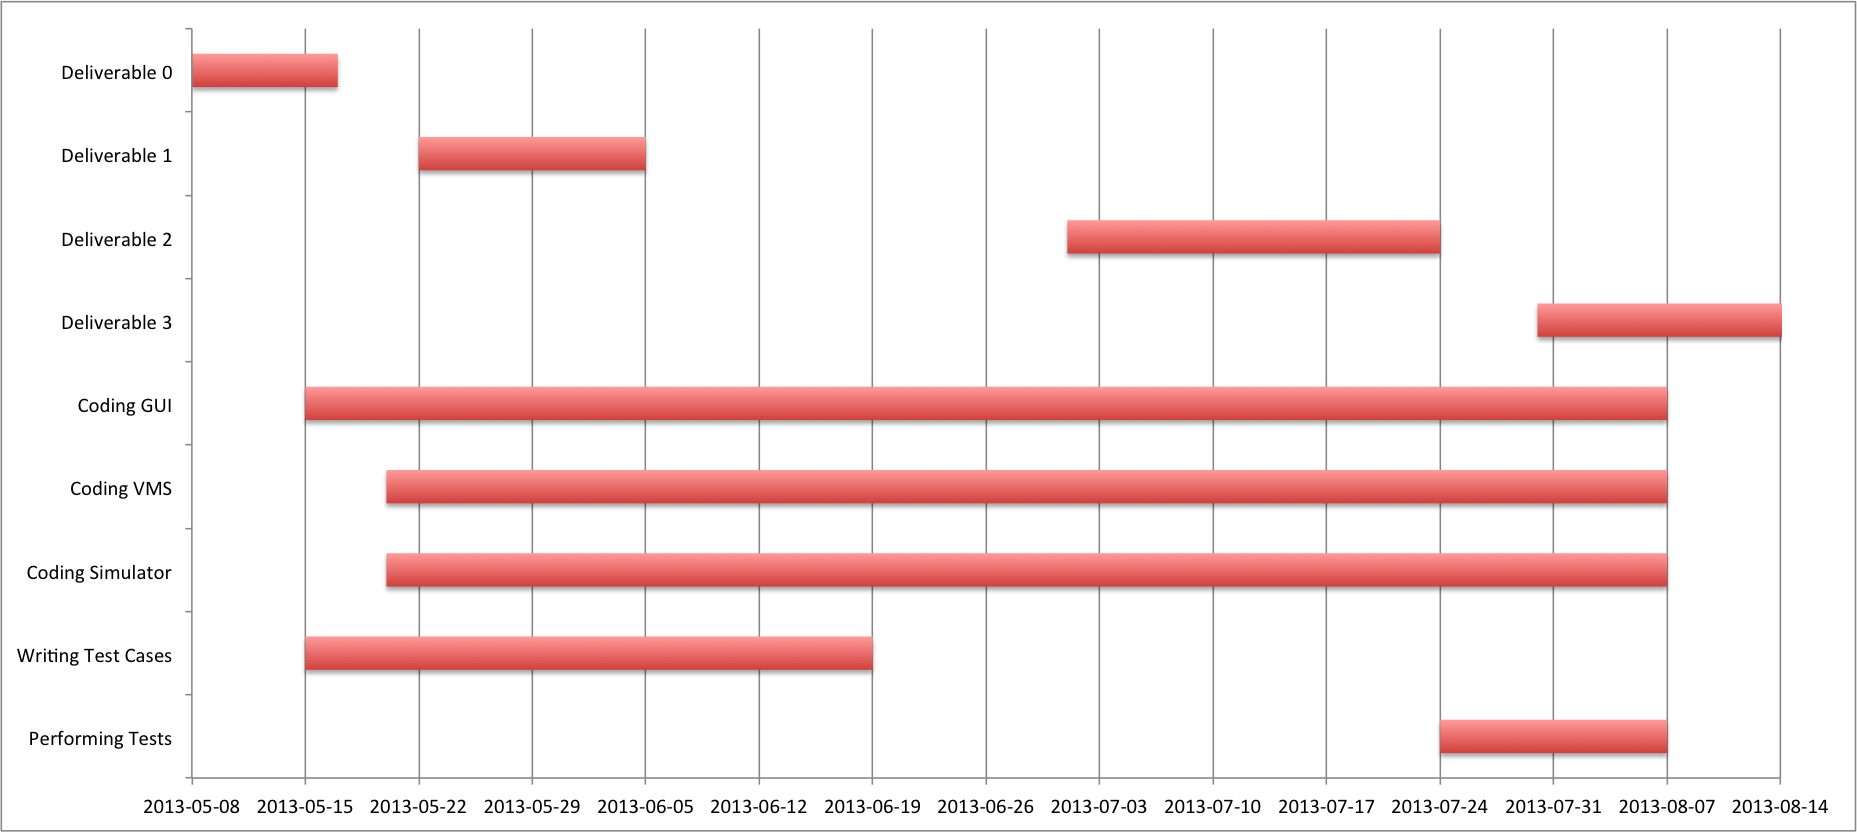
\includegraphics[scale=0.55]{charts/GanttChart.png}
\end{figure}

% Taken from last deliverable with only minor changes. Costs may have to be recalculated.
\begin{description}
  \item[Simulator program:] \$150, cost to code and implement.
  \item[VMS program:] \$150, cost to code and implement.
  \item[Graphical User Interface:] \$100, cost to design, code, and implement.
  \item[Unit test suite:] \$200, cost to write test cases and perform testing.
  \item[Documentation:] \$250, includes all customer deliverables and internal documentation.
  \item[Final integration:] \$90
  \item[Buffer:] \$160
  \item[Total Cost:] \$1100
\end{description}

\paragraph{Basis} Costs have been calculated based on the amount of man hours spent working on project (at a normal approximate labor cost of \$15 an hour). There was no cost associated with tools, because all tools used were either freely available or were provided by the University.

\end{document}
